\documentclass[12pt,twoside]{article}
\usepackage[spanish]{babel} % espanol
\usepackage[utf8]{inputenc} % acentos sin codigo
\usepackage{enumerate} % enumerados
\usepackage{float}
\usepackage[utf8]{inputenc}
\usepackage[spanish]{babel}
\usepackage{amsmath, amssymb}
\usepackage{amsmath}
\usepackage[active]{srcltx}
\usepackage{amssymb}
\newcommand{\addfigure}[4]{
        \begin{figure}[htbp!]
            \begin{center}	
                \fbox{\includegraphics[width=#1\textwidth]{#2}}
                \caption{#4}
                \label{#3}
            \end{center}
        \end{figure}
  }
\usepackage{amscd}
\usepackage{listings}
\usepackage[T1]{fontenc}
\usepackage{makeidx}
\usepackage{amsthm}
\usepackage{algpseudocode}
\usepackage{algorithm}
\usepackage{algorithmicx}
\usepackage{graphicx}
\usepackage{vmargin}
\graphicspath{ {images/} }
\renewcommand{\baselinestretch}{1}
\setcounter{page}{1}
\setlength{\textheight}{21.6cm}
\setlength{\textwidth}{14cm}
\setlength{\oddsidemargin}{1cm}
\setlength{\evensidemargin}{1cm}
\setlength{\intextsep}{0pt}
\thispagestyle{empty}
\setpapersize{A4}
\setmargins{2.5cm}       % margen izquierdo
{1.5cm}                        % margen superior
{16.5cm}                      % anchura del texto
{23.42cm}                    % altura del texto
{10pt}                           % altura de los encabezados
{1cm}                           % espacio entre el texto y los encabezados
{0pt}                             % altura del pie de página
{2cm}                           % espacio entre el texto y el pie de página
\title{Practica 9}
\date{}
\begin{document}
\centerline{\bf An\'alisis de Algoritmos, Sem: 2019-1, 3CV1, Pr\'actica 9, 28/11/2018}
\centerline{}
\centerline{}
\begin{center}
\Large{\textsc{Pr\'actica 9: Estrategia Greedy.}}
\end{center}
\centerline{}
\centerline{\bf {Hern\'andez Castellanos C\'esar Uriel, Aguilar Garcia Mauricio}}
\centerline{}
\centerline{Escuela Superior de C\'omputo}
\centerline{Instituto Polit\'ecnico Nacional, M\'exico}
\centerline{$uuriel12009u@gmail.com, mauricio.aguilar.garcia.90@gmail.com$}
\newtheorem{Theorem}{\quad Theorem}[section]
\newtheorem{Definition}[Theorem]{\quad Definition}
\newtheorem{Corollary}[Theorem]{\quad Corollary}
\newtheorem{Lemma}[Theorem]{\quad Lemma}
\newtheorem{Example}[Theorem]{\quad Example}
\bigskip
\textbf{Resumen: } Se implementa el algoritmo para la compresión de cadenas por medio de códigos Huffman y también la descompresión del mismo, mostrando como se implementa por la Estrategia Greedy.
\\ 
\\
\textbf{Palabras Clave: } Algoritmo, Complejidad, Compresión, Estrategia, Greedy, Códigos, Huffman, Heap y Árbol.

\section{Introducción}
\label{sec:introduction}

En ciencias de la computación y teoría de la información, la codificación Huffman es un algoritmo usado para compresión de datos. El término se refiere al uso de una tabla de códigos de longitud variable para codificar un determinado símbolo (como puede ser un carácter en un archivo), donde la tabla ha sido rellenada de una manera específica basándose en la probabilidad estimada de aparición de cada posible valor de dicho símbolo. Fue desarrollado por David A. Huffman mientras era estudiante de doctorado en el MIT, y publicado en "A Method for the Construction of Minimum-Redundancy Codes".

La codificación Huffman usa un método específico para elegir la representación de cada símbolo, que da lugar a un código prefijo (es decir, la cadena de bits que representa a un símbolo en particular nunca es prefijo de la cadena de bits de un símbolo distinto) que representa los caracteres más comunes usando las cadenas de bits más cortas, y viceversa. Huffman fue capaz de diseñar el método de compresión más eficiente de este tipo: ninguna representación alternativa de un conjunto de símbolos de entrada produce una salida media más pequeña cuando las frecuencias de los símbolos coinciden con las usadas para crear el código. Posteriormente se encontró un método para llevar esto a cabo en un tiempo lineal si las probabilidades de los símbolos de entrada (también conocidas como "pesos") están ordenadas.

Para un grupo de símbolos con una distribución de probabilidad uniforme y un número de miembros que es potencia de dos, la codificación Huffman es equivalente a una codificación en bloque binaria, por ejemplo, la codificación ASCII. La codificación Huffman es un método para crear códigos prefijo tan extendido que el término "codificación Huffman" es ampliamente usado como sinónimo de "código prefijo", incluso cuando dicho código no se ha producido con el algoritmo de Huffman.

Aunque la codificación de Huffman es óptima para una codificación símbolo a símbolo dada una distribución de probabilidad, su optimalidad a veces puede verse accidentalmente exagerada. Por ejemplo, la codificación aritmética y la codificación LZW normalmente ofrecen mayor capacidad de compresión. Estos dos métodos pueden agrupar un número arbitrario de símbolos para una codificación más eficiente, y en general se adaptan a las estadísticas de entrada reales. Este último es útil cuando las probabilidades no se conocen de forma precisa o varían significativamente dentro del flujo de datos. \cite{pal}
\vspace{5 mm}
\begin{figure}[H]
\centering
\includegraphics[scale=0.4]{img_cinco/Huffman.jpg}
\caption{David Huffman}
\end{figure}

\section{Conceptos Básicos}

\subsection{Estrategia greedy}
Los algoritmos que se obtienen aplicando este esquema se denominan, por extensión, algoritmos voraces. El
esquema forma parte de una familia de algoritmos mucho más amplia denominada
ALGORITMOS DE BUSQUEDA LOCAL de la que también forman parte, por ejemplo, el
método del gradiente, los algoritmos Hill-Climbing, los algoritmos genéticos o los
Simulated Annealing.\\
\\
Antes de ver propiamente el esquema de resolución, comenzaremos por
caracterizar de forma general las condiciones que deben cumplir los problemas que
son candidatos a ser resueltos usando un algoritmo voraz:\\
\\
El problema a resolver ha de ser de optimización  y debe existir una
función, la función objetivo, que es la que hay que minimizar o maximizar.
      \\
Existe un conjunto de valores posibles para cada una de las variables de la
función objetivo, su dominio.\\
\\
Puede existir un conjunto de restricciones que imponen condiciones a los
valores del dominio que pueden tomar las variables de la función objetivo.\\
La solución al problema debe ser expresable en forma de secuencia de
decisiones y debe existir una función que permita determinar cuándo una
secuencia de decisiones es solución para el problema (función solución).\\
\\
Entendemos por decisión la asociación a una variable de un valor de su domino.
Debe existir una función que permita determinar si una secuencia de decisiones
viola o no las restricciones, la función factible.\cite{cota}

\subsection{Aplicaciones}
.\\
  Planificación de tarea\\
  Cajeros\\
  Caminos mínimos en grafos\\
  Árbol generador minimal\\
  Códigos Huffman y compresión de datos\\
  Construcción de árboles de decisión\\
  Heuristica Greedy\\
\\
\subsection{Algoritmos} 
\subsubsection{Huffman}
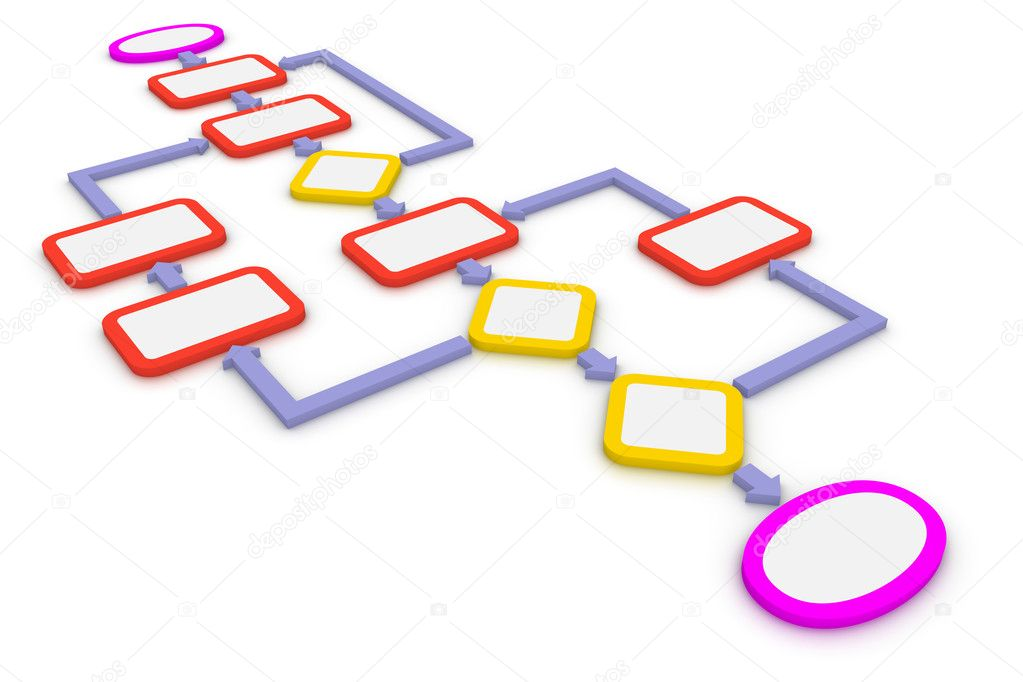
\includegraphics[height=.4\textwidth]{img_nueve/algoritmo.png}
\\
El algoritmo consiste en la creación de un árbol binario que tiene cada uno de los símbolos por hoja, y construido de tal forma que siguiéndolo desde la raíz a cada una de sus hojas se obtiene el código Huffman asociado a él.\\

Se crean varios árboles, uno por cada uno de los símbolos del alfabeto, consistiendo cada uno de los árboles en un nodo sin hijos, y etiquetado cada uno con su símbolo asociado y su frecuencia de aparición.\\
\\
Se toman los dos árboles de menor frecuencia, y se unen creando un nuevo árbol. La etiqueta de la raíz será la suma de las frecuencias de las raíces de los dos árboles que se unen, y cada uno de estos árboles será un hijo del nuevo árbol. También se etiquetan las dos ramas del nuevo árbol: con un 0 la de la izquierda, y con un 1 la de la derecha.\\
\\
Se repite el paso 2 hasta que sólo quede un árbol.\\
\\
Con este árbol se puede conocer el código asociado a un símbolo, así como obtener el símbolo asociado a un determinado código.
Para obtener el código asociado a un símbolo se debe proceder del siguiente modo:\\
\\
1 Comenzar con un código vacío.\\
2 Iniciar el recorrido del árbol en la hoja asociada al símbolo.\\
3 Comenzar un recorrido del árbol hacia arriba.\\
4 Cada vez que se suba un nivel, añadir al código la etiqueta de la rama que se ha recorrido.\\
5 Tras llegar a la raíz, invertir el código.\\
6 El resultado es el código Huffman deseado.\\
Para obtener un símbolo a partir de un código se debe hacer así:
\\
1 Comenzar el recorrido del árbol en la raíz de éste.\\
2 Extraer el primer símbolo del código a descodificar.\\
3 Descender por la rama etiquetada con ese símbolo.\\
4 Volver al paso 2 hasta que se llegue a una hoja, que será el símbolo asociado al código.\\
En la práctica, casi siempre se utiliza el árbol para obtener todos los códigos de una sola vez; luego se guardan en tablas y se descarta el árbol.
\\
Se tiene el código implentado de huffman, Figura 1.
\vspace{10 mm}
\addfigure{.8  }{img_nueve/huffmanCodes}{fig:SP}{Implementación de los códigos de Huffman}
\section{Experimentación y Resultados}
\subsection{Códigos de Huffman}
Para realizar esta prueba se hizo uso del archivo ``archivo.txt'' el cual su contenido es ``hola Mundo, éste es un archivo de prueba para compresion por medio de Huffman.'' y tiene un peso inicial de 79 bytes. Este archivo lo vamos a dar como entrada al programa ``\textit{comprimir.py}'' el cual se encargará de hacer la compresión, como se ve la Figura 2.\\
\addfigure{.8  }{img_nueve/runProgram}{fig:SP}{Salida del programa}\\
Como se puede apreciar en la figura anterior, se generaron los archivos \textit{``archivoCodificado.txt'' (Figura 3), ``codificación.txt'' (Figura 4) y ``frecuencias.txt'' (Figura 5)} y en ellos se aprecia que el tamaño del archivo codificado es de 43 bytes, por lo que se consiguió una compresión en un 54.43\% del archivo original.


\addfigure{.8  }[H]{img_nueve/salCod}{fig:SP}{Contenido del archivo archivoCodificado.txt.}
\addfigure{.6 }[H]{img_nueve/salCodes}{fig:SP}{Contenido del archivo codificacion.txt.}
\addfigure{.8  }[H]{img_nueve/freqs}{fig:SP}{Contenido del archivo frecuencias.txt.}
\\
Ahora para corroborar que se comprimió de manera correcta y no hay perdida de información vamos a descomprimir el archivo codificado. En este caso el archivo codificado junto con el archivo de codificación forman la como entrada al programa ``\textit{descomprimir.py}'' el cual se encargará de hacer la descompresión, como se ve la Figura 6.\\

\addfigure{.8  }{img_nueve/runProgramD}{fig:SP}{Salida del programa ingresando archivo.txt.}\\

Como se puede apreciar en la figura anterior, se generó el archivo \textit{``archivoDecodificado.txt''}, y también se puede observar que el tamaño del archivo decodificado es de 79 bytes, que es el mismo que el de \textit{``archivo.txt''} el cual fue nuestro archivo de entrada.\\
Para checar que efectivamente es la misma información, simplemente imprimimos el contenido del archivo decodificado y para ser más estrictos nos auxiliamos del programa \textit{diff} el cual nos imprime las diferencias que encuentre entre dos archivos o nada en caso de que sean iguales, como se puede ver en la Figura 7.\\
\addfigure{.8  }{img_nueve/salOri}{fig:SP}{Contenido del archivo archivoCodificado.txt.}
\\
\section{Conclusiones}
\subsection{Conclusión de Hernández Castellanos César Uriel}
	El método que se implementó en la práctica es muy poderoso, ya que trabaja bien en muchos algoritmos, cómo lo es Árbol de expansión mínima, Algoritmo de Dijkstra para el camino más corto desde  una fuente etc.\\
	
	Es importante verificar que el problema exhiba la optical -subestructure property antes de intentar implementar una estrategia Greedy.\\
	
	Una estrategia Greedy puede llegar a ser fácil de implementar, pero puede fallar.\\
	
	En cuanto a la práctica, no nos resultó complicada desarrollarla, ya que en años anteriores cuándo cursabamos estructuras de datos, la elaboramos como proyecto final.
	
\subsection{Conclusión Mauricio Ahuilar Garcia }
    Los algoritmos greedy funcionan de una manera muy eficiente puesto que solo toman decisiones localmente, en esta práctica pude ver como se implementa este paradigma enfocado en la codificación por medio de códigos huffman, y pude notar que generalmente éste tipo de algoritmo es sencillo y fácil de entender puesto que las condiciones tienden a ser simples.     	
\subsection{Conclusiones generales}
    	En esta práctica pudimos verificar que hay problemas que se pueden resolver por algoritmos Greedy y que tienen soluciones muy elegantes, ya que son fáciles de programar y de entender , como los códigos de Huffman que nos permiten comprimir un archivo de una manera eficiente, ya que los códigos de Huffman son únicos y no tienen prefijos en común lo que facilita mucho el análisis del mismo.

\begin{thebibliography}{9}
\bibitem{pal}
  D.A. Huffman, A method for the construction of minimum-redundancy codes", Proceedings of the I.R.E., sept 1952, pp 1098-1102
 \bibitem{cota}
 Cs.upc.edu. (2017).[online] Available at: http://www.cs.upc.edu/~mabad/ADA/curso0708/GREEDY.pdf.
\end{thebibliography}
\end{document}